
\section{End-User Development}
\subsection{Begriffserklärung}
Im 21. Jahrhundert verwendet fast jeder Berufszweig Computer-Gestützte Systeme, um effizienteres Arbeiten zu ermöglichen. Es ist allerdings unmöglich jegliche Software genau auf den Use-Case zu zuschneiden, da die Kapazitäten an professionellen Software-Ingenieuren schlichtweg nicht ausreicht. Endnutzer sollen diese Lücke füllen. Endnutzer sind Software-Nutzer, die sich intensiv mit ihrer Anwendungsdomäne beschäftigen und dafür tagtäglich Software verwenden aber nur Laienhaft mit Computerprogrammierung vertraut sind. In 2005 wurde von \cite{Scaffidi2005eudnumbers} geschätzt, dass die Anzahl der Endnutzer auf über 90 Millionen (in den Vereinigten Staaten) im Jahr 2012 anwachsen wird. Der Grund hierfür ist einfach: die stetige Diversifikation von Geschäftsfeldern und Spezialisierung der Anwendungsfälle von Software steht einer geringen Anzahl ausgebildeter Software Ingenieure gegenüber. Endnutzer unterscheiden sich von Entwicklern, indem sie oftmals wenig Verständnis für Programmierung haben aber starkes Domänenwissen besitzen. Ihr Ziel ist es nicht allgemeingültige Softwareartefakte zu erstellen, sondern bestehende Software auf die individuellen Bedürfnisse zuschneiden.

Die Begrifflichkeit des \acf{EUD} selbst wuchs aus ursprünglich aus dem Thema des \ac{EUP} und \ac{EUC}. Unter dem Begriff \ac{EUP} wurde zu Beginn Prgrammier- und Scriptsprachen verstanden, welche von der unterliegenden Hardware abstrahierten und Nicht-Software-Ingenieuren erstmals erlaubte, eigene Programme zu entwickeln und bestehende Softwaresysteme zu erweitern. In den 1970er und 1980er wurde aus diesem  Paradigma \ac{EUC}, unter dem man Programmiersprachen der vierten Generation zusammenfasst (bspw. SQL). Diese Sprachen besitzen ein wesentlich höheres Abstraktionsniveau von der darunterliegenden Programmlogik als traditionelle Programmiersprachen. Sprachen wie SQL tauschen ihre Allgemeingültigkeit (bspw. ist SQL nicht Touring-Komplett) gegen ein auf die Domäne zugeschnittenes Programmierparadigma. Je nach Literaturquelle wird \ac{EUP} als vorherige Evolutionsstufe von \ac{EUD} gesehen oder oftmals Synonym mit \ac{EUD} verwendet. \ac{EUD} sollte daher als eine Obermenge der Paradigmen angesehen werden, dies wird besonders offensichtlich wenn Nachfolgeparadigmen wie \ac{EUSE} das \ac{EUD} Modell um einen Softwareentwicklungszyklus erweitert (\cite{Ko2011EUSE}).

Die für \ac{EUD} am weitesten verbreitete Definition ist von \cite{Lieberman.2006} und lautet wie folgt:

''\textit{End-User Development can be defined as a set of methods, techniques, and tools that allow users of software systems, who are acting as non-professional software developers, at some point to create, modify or extend a software artifact.}''

\ac{EUD} umschließt alle Prozesse, Werkzeuge und (Programmier-)Paradigmen, welche es End-Nutzern (bspw. Domänen-Experten, Studenten, Designer) abstrahiert von Low-Level Programmierkenntnissen Software zu erzeugen, zu warten und zu erweitern. Von \cite{ko2004six} wurden anhand einer Nutzerstudie sechs Barrieren ermittelt, welche dem Erfolg eines \ac{EUD}-Werkzeugs im Weg stehen kann:
\begin{itemize}
    \item \textbf{Design-Barriere}: ''\textit{Ich weiß nicht wie man das Problem definieren kann.}'' Tritt auf wenn ein Endnutzer grundsätzliche Probleme hat, das Problem in einer Form zu designen, in der es vom Computer verarbeitet werden kann.
    \item \textbf{Auswahls-Barriere}: ''\textit{Ich kann das Problem definieren aber weiß nicht, welches Werkzeug mir dabei behilflich ist.}'' Der Endnutzer weiß wie er das Problem definieren soll, nicht aber, welche konkreten Elemente des \ac{EUD}-Werkzeugs ihm dabei helfen es zu lösen.
    \item \textbf{Koordinations-Barriere}: ''\textit{Ich weiß, welche Werkzeuge ich benutzen muss aber nicht wie ich sie miteinander agieren lasse.}'' Der Endnutzer hat in diesem Fall Schwierigkeiten, die einzelnen Komponenten des \ac{EUD}-Werkzeugs miteinander zu kombinieren um das Problem zu lösen. 
    \item \textbf{Verwendungs-Barriere}: ''\textit{Ich weiß, welches Werkzeug ich benutzen muss aber nicht wie es funktioniert.}'' Das \ac{EUD}-Werkzeug oder eine Teilkomponente ist nicht explizit in der Funktion, die es bereitstellt und erlaubt dem Endnutzer Fehler zu begehen. 
    \item \textbf{Verständnis-Barriere}: ''\textit{Das Werkzeug hat sich nicht so verhalten, wie es erwartet hatte.}'' Hierbei herscht eine kognitive Diskrepanz zwischen dem Verhalten dass der Endnutzer von einer \ac{EUD}-Notation erwartet, und wie sie sich tatsächlich verhält.
    \item \textbf{Informations-Barriere}: ''\textit{Ich glaube, ich weiß warum es sich anders verhalten hat aber ich habe keine Möglichkeit, dies zu überprüfen.}''  Das \ac{EUD}-Werkzeug macht (Fehl-)Verhalten ist für den Endnutzer schwer nachvollziehbar.
\end{itemize}
Um diese Barrieren zu überwinden benötigen \ac{EUD}-Werkzeuge laut \cite{ko2004six} eine passende Design-Metapher. Eine solche Metapher sollte anhand der Komplexität und Natur der Domäne gebunden sein. Eine solche Metapher soll Mensch-Bezogen sein, die sechs Barrieren beachten, Abstrakt von Programmlogik und möglichst nah an der Domäne sein, sodass der Endnutzer sinnvolle Analogien zur realen Welt ziehen kann können. 

\subsection{EUD Design}\label{sec:loesungsans}
\begin{figure}[H]
    \centering
    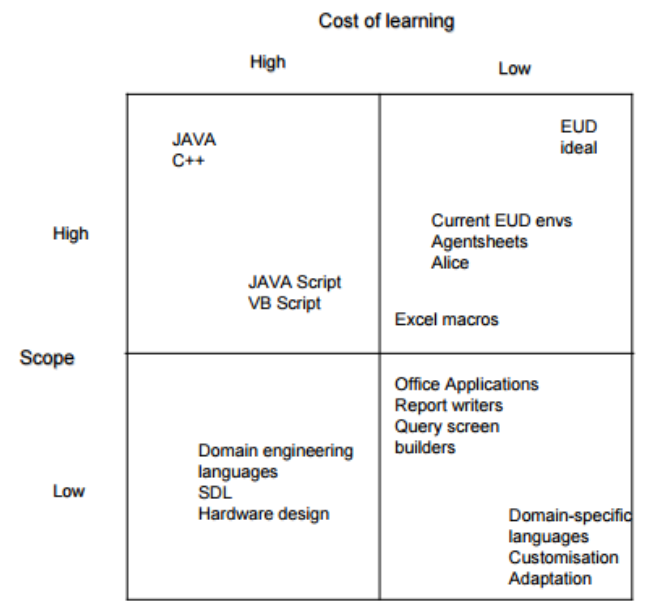
\includegraphics[width=0.7\textwidth]{bilder/chapter2/eudmatrix.png}
    \caption{Umfang des Anwendungsbereichs und Höhe des Lernaufwands unterschiedlicher \ac{EUD}-Werkzeuge gegenübergestellt.}
    \label{fig:kompvslern}
\end{figure}
Es gibt zwei Dimensionen, die bei der Erstellung eines \ac{EUD}-Werkzeug zu beachten sind: \textit{Anwendungsbereich} und \textit{Lernaufwand} (\cite{fischer2004meta}). In Abbildung \ref{fig:kompvslern} werden vier Quadranten gezeigt, welche Repräsentanten von Softwareerstellungs-Werkzeugen in ihrer Anwendungsbereich (Abbildungsvermögen des Werkzeugs) und ihrem Lernaufwand (zeitlicher Aufwand zum Erlernen des Werkzeugs) gegenüberstellt. Im Quadrant, der eine großen Anwendungsbereich abdeckt und einen hohen Lernaufwand an den Nutzer stellt, sind die klassischen Entwicklungswerkzeuge wie \texttt{C++} zu finden. Die Werkzeuge in diesem Quadrant sind nur meist nicht Domänen-gebunden und geben nur wenig Vorgaben unter welchem Paradigma sie verwendet werden müssen. Diese Flexibilität hat allerdings ihren Preis, den der Endnutzer muss über Monate und Jahre lernen, mit dieser Abstraktion umgehen zu können. Es existieren auch Werkzeuge mit einer wohl definierten Abbildungsvermögen (geringer Scope) und einer steilen Lernkurve. \acp{HDL} repräsentieren einen Vertreter dieses Quadranten. Ihre Komplexität geht einher mit der Einzigartigkeit der Domäne und der benötigten Spezialisierung des Endnutzers. \ac{EUD}-Werkzeuge sollten sich laut \cite{fischer2004meta} im Quadranten mit geringem Lernaufwand und großer Anwendbarkeit befinden. Ein solchen \ac{EUD}-Werkzeug ist allerdings nicht trivial umzusetzen. Wie schon im vorherigen Kapitel angesprochen, benötigen \acp{EUD}-Werkzeuge eine, auf die Domäne abgestimmte, Design-Metapher. Aus diesem Grund ist es fraglich ob ein solches, ideales \ac{EUD}-Werkzeug existieren kann.

\subsubsection{Cognitive Dimensions}
\begin{table}[h]
\centering
\begin{tabularx}{\textwidth}{lX}
\hline
\rowcolor[HTML]{EFEFEF} 
Dimension                 & Definition                                           \\ \hline
Viskosität                & Wiederstand gegenüber Veränderung                    \\ \hline
Sichtbarkeit              & Sichtbarkeit von Komponenten                         \\ \hline
Vorzeitige Festlegung     & Feste Vorgaben bei Interkationsreihenfolge           \\ \hline
Unsichtare Abhängigkeiten & Sichtbarkeit der Abhängigkeiten zwischen Komponenten \\ \hline
funktionale Aussagekraft  & Ersichtlichkeit der Funktionalität einer Komponente  \\ \hline
Fehleranfälligkeit        & Aktive/Passive Verhinderung von Fehlern              \\ \hline
Abstraktionen             & Qualität der Abstraktion von Datentypen/Komponenten  \\ \hline
Sekundäre Notation        & Zusätzliche Informationen unabhängig Notation        \\ \hline
Domänennähe               & Nähe der Design-Metaphern zur Domäne                 \\ \hline
Konsistenz                & Ähnliche Semantiken besitzen ähnliche Syntax         \\ \hline
Zerstreutheit             & Ausdrucksstärke der Notation                         \\ \hline
Mentaler Aufwand          & Kognitive Kosten der Notation                        \\ \hline
Endgültigkeit             & Finalität von Interaktionen                          \\ \hline
Vortwährende Evaluation   & Übersicht des eigenen Voranschreitens                \\ \hline
\end{tabularx}
\caption{Cognitive Dimensions laut [\cite{blackwell2003notational}]}
\label{tab:cognitivedimensions}
\end{table}
\acl{CD} ist ein in \cite{blackwell2003notational} vorgestelltes Framework um die Notation von (visuellen) Programmiersprachen zu bewerten. Nach \cite{blackwell2003notational} handelt es sich bei \ac{CD} nicht um eine konkrete Validierungsmethode, sondern vielmehr um ein Rahmenwerk von Vokabeln um die Usability einer Programmiersprache zu diskutieren. Vokabeln dieses Rahmenwerks werden kognitive Dimensionen genannt. In Tabelle \ref{tab:cognitivedimensions} kann eine vollständige Aufzählung sämtlicher kognitiver Dimensionen eingesehen werden. \ac{CD} verfolgt im Allgemeinen folgende Ziele:

\begin{itemize}
    \item Designer ermöglichen gezielte Aspekte (mit sich selbst) diskutieren und vergleichen zu können.
    \item Kompromisse und Schwerpunkte zwischen den verschiedenen Aspekten zu setzen.
    \item Erlaubt es durch groben Zügen über die Usability einer Sprache zu urteilen ohne sich in Detail zu verlaufen (''\textit{death by detail}'')
\end{itemize}

\ac{CD} schreibt laut \cite{blackwell2003notational} keine explizite Methode vor, wie verwendet werden soll. In der Praxis findet \ac{CD} als Basis von Fragebögen (z.B. \cite{EBobkowska.2003}, \cite{Wijayarathna.}) und als Grundlage für \textit{Cognitive Walkthroughs} (Evaluation anhand von Expertenmeinung, welche Handlungsabläufe innerhalb eines Werkzeuges durchspielen und bewerten) Verwendung (z.B. \cite{blackwell2000cognitive}). 

\begin{table}[h]
\centering
\begin{tabularx}{\textwidth}{lXX}
\hline
\rowcolor[HTML]{EFEFEF} 
Aktivität           & Definition                                                               & Beispiel\\ \hline
Suchen              & Finden von Informationen innerhalb der Notation                          & Finden eines Wertes innerhalb einer Tabellenzelle\\ \hline
Exploratives Design & Design eines Artefakts ohne einen festen Lösungsansatz                   & Live-Reloading, Skizzieren, etc.\\ \hline
Inkrementieren      & Hinzufügen von Informationen ohne die Struktur der Notation zu verändern & Hinzufügen von Funktionen zu einem Programm\\ \hline
Transkribieren      & Transformieren einer Information von einer Notation in eine Andere       & Kopieren einer Formel von einem Buch in eine Tabelle\\ \hline
Modifizieren        & Ändern einer Notationsstruktur ohne Informationen hinzuzufügen           & Layout einer Tabellenkalkulation ändern \\ \hline
\end{tabularx}
\caption{Aktivitäten innerhalb eines \ac{EUD}-Werkzeugs anhand \cite{green2000instructions}}
\label{tab:cogaktivitaeten}
\end{table}

Neben den in Tabelle \ref{tab:cognitivedimensions} definierten kognitiven Dimensionen, wird in \cite{green2000instructions} noch eine Reihe von \textit{User Activities} (Tabelle \ref{tab:cogaktivitaeten}) aufgezeigt. Diese Aktivitäten des \ac{EUD}-Werkzeugs erlauben dem Endnutzer, Softwareartefakte zu erstellen und zu modifizieren. Ziel dieser Aktivitäten ist es \textit{Trade-Offs} zwischen den kognitiven Dimensionen schärfer rationalisieren zu können. Beispielsweise ist die Viskosität beim Inkrementieren eines Wertes in den meisten Fällen sehr wichtig beim Suchen von Werten spielt es allerdings nur eine nebensächliche Rolle. 

\section{State-of-the-Art}\label{subsec:stateoftheart}
Im Folgenden werden populäre \ac{EUD}-Paradigmen untersucht. Da \ac{IoT} als Technologie noch selbst in einer frühen Entwicklungsphase befindet, ist die Anzahl von produktiv eingesetzten \acp{EUD} in diesem Bereich noch stark begrenzt. Im Folgenden werden \ac{EUD}-Ansätze, die für die \ac{IoT}-Domäne entworfen wurden, diskutiert.

\subsection{Programming-by-Demonstration}
\paragraph{Beschreibung} \acf{PBD} ist eine weit verbreitetes \ac{EUD}-Paradigma zum Programmieren von repetitiven Arbeitsvorgängen (\cite{cypher1993pbd}). Auch Programming-by-Example genannt, nimmt der Endnutzer eine Reihe von Arbeitsschritten innerhalb der verwendeten Software manuell vor. Diese Arbeitsschritte werden aufgenommen und von dem \ac{PBD}-System in einen Algorithmus transformiert. Dieser Algorithmus erlaubt es dem Computer autonom die gleichen Arbeitsschritte auf ähnlich strukturierten Datensätzen nachzuahmen. Dadurch wird erreicht, dass nicht Software-affine Endnutzer ohne das explizite Nutzen einer Programmiersprache oder \ac{GUI}, Algorithmen definieren können.

\paragraph{Funktionsweise} Wie in \cite{cypher1993pbd} beschrieben, ist das einfachste Beispiel für die Implementierung von \ac{PBD}-Systemen, ein Makrorekorder. Makrorekorder sind ein fester Bestandteil vieler weit verbreiteter Software-Systemen (bspw. Excel oder Adobe Photoshop). Sie erlauben es dem Nutzer repetitive Vorgänge aufzunehmen um Sie dann von der Software auf zukünftige Arbeitspakete replizieren zu lassen. Wie \cite{cypher1993pbd} hier anmerkt, sind solche Ansätze zwar einfach für den Endnutzer zu erlernen aber auch stark in ihrer Flexibilität und Ausdrucksweise eingeschränkt. In der Literatur gibt es verschiedene Ansätze diese Einschränkung mindestens partiell zu umgehen. Beispielsweise kann die Makro-Aufzeichnung als (visueller) Programmcode angezeigt werden. Dieser Programmcode kann dann vom Endnutzer modifiziert und generalisiert werden, um für eine größere Bandbreite von Datensätzen nutzbar zu sein.

\begin{figure}[h]
    \centering
    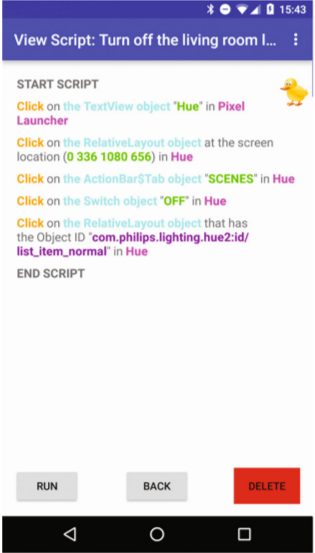
\includegraphics[width=0.3\textwidth]{bilder/chapter2/epidosite__example.png}
    \caption{\textit{EPIDOSITE}-Skript, das Interaktionen mit einer \ac{IoT}-Lampe beschreibt}
    \label{fig:epidositeexample}
\end{figure}

\paragraph{EPIDOSITE} Ein Beispiel für die Integration des \ac{PBD}-Paradigmas ist die, von \cite{li2017programming} vorgeschlagene, \textit{EPIDOSITE}-Plattform. Hierbei kann ein Makrorekorder, welcher auf einem Smartphone installiert ist, eine Abfolge von App-Interaktionen mit IoT-Systemen (bspw. Phillips Hue) aufnehmen. Einzelne Interaktionen können dann verkettet werden um komplexere Szenarien zu beschreiben. Grundsätzlich beschreibt der Endnutzer durch seine aufgenommenen Interaktionen \textit{Triggers} (dt. ''Auslöser/Bedingungen'') und \textit{Actions} (dt. ''Aktionen''). In einem Review-Prozess kann der Benutzer eine Skript (siehe Abbildung \ref{fig:epidositeexample}), welches der Makroaufnahme entspricht, überprüfen und gewünschte Änderungen vornehmen. Um die Interoperabilität und Funktionalität des Systems zu erhöhen lässt \textit{EPIDOSITE} dem Benutzer zu, virtuelle \textit{Services} über \textit{IFTTT} anzusprechen. 

\paragraph{Wertung} Der primäre \textbf{Vorteil} dieses Ansatzes ist der des \ac{PBD}-Paradigmas: ohne jegliche Programmierkenntnisse lässt sich ein \ac{IoT}-Systeme steuern bzw. im Verbund orchestrieren. Ein weiterer Vorteil von \textit{EPIDOSITE} bszw. \ac{PBD} sieht \cite{cypher1993pbd} darin, dass die Programmierung nicht von dem Interface, in der das Programm ausgeführt wird, getrennt ist (''\textit{Programming within the User Interface}''). Dieses Überlagern von \ac{EUD}- und Anwendungs-\textit{UI} reduziert die kognitive Dissonanz zwischen Entwicklung und Anwendung, welche bei Programmiersprachen vorherrscht. Somit erspart sich das \ac{PBD}-Paradigma in einfachen Anwendungen eine Abstraktionsebene. Als größte Herausforderung sieht \cite{cypher1993pbd} für \ac{PBD}-Systeme, die implizierte Absichten des Users herauszufinden. Selektiert man Beispielsweise in \textit{EPIDOSITE} die Temperatur eines Raums (um bspw. die Heizung einzuschalten) ist das \ac{EUD}-System erst einmal für unklar, welche genaue Bedingung der Benutzer damit verknüpft (''Heizung anschalten bei: kleiner 20°C? kleiner-gleich 20°C? etc.''). Des Weiteren stellen simple Makroaufnahmen sequentielle Programmabläufe dar. Um komplexere Konstrukte (komplexe Bedingungen, Umwandeln von Datensätzen, Schleifen) zu schaffen, welche in einem \ac{IoT}-Szenario durchaus erdenklich sind, werden zusätzliche Funktionalitäten benötigt. Ein weiterer Nachteil, der von \cite{li2017programming} beschrieben wird ist, dass die Sichtbarkeit von Fehlern im Programmablauf stark eingeschränkt ist. Diese Undurchsichtigkeit schränkt die Usability des Werkzeugs eins. Des Weiteren fehlt \textit{EPIDOSITE} eine Möglichkeit erstellte Skripte zu simulieren. Würde der Benutzer eine Aktion an eine Bedingung an die Tageszeit knüpfen, müsste er die Uhr seines Smartphones verstellen um das Skript zu überprüfen. Dies erschwert das Programmieren von Aktionen, die an schwer manipulierbare Umgebungsvariablen (bspw. Temperatur, Helligkeit, etc.) gebunden sind.

\subsection{\acl{TAP}}

\paragraph{Definition} \ac{TAP} oder auch \textit{Rule-based Programming} stellt eine weitere, populäre Methode im \ac{EUD} für \ac{IoT}-Applikationen dar. Es handelt sich hierbei um ein stark vereinfachtes Programmierparadigma, welches dazu genutzt wird, Ereignisse zwischen mehreren Informationsquelle (z.B. Smart-Objects) zu lenken und sie somit kompositionieren (\cite{ur2014practical}). Bei \ac{TAP} spezifiziert der Endnutzer Sammlungen von Regeln, welche jeweils aus einer Aktion (Action) besteht, die vom System durchgeführt werden soll, falls ein Signal eintritt, das eine definierte Bedingung (Trigger) erfüllt. 

\paragraph{Funktionsweise} Ein typische \ac{TAP}-System besteht grundsätzlich zwei Elementen: Bedingung (Trigger) und Actions (Aktionen). Trigger können laut \cite{huang2015supporting} zwei Formen annehmen: Event (Einzigartig; bspw. ''Knopf wurde gedrückt'') oder State (Fortwährend; bspw. ''Die Sonne scheint''). Die resultierende Aktion kann ein Signal in drei verschiedenen Ausprägungen annehmen: Instant (analog zu Event), Sustained (analog zu State) und Extended (Temporär; bspw. ''Abschalten von Licht nach 2 Minuten''). Diese beiden Elemente (Trigger und Action) werden dann durch ein \ac{EUD}-Werkzeug auf visueller oder textueller Ebene zu Regeln zusammengefasst, welche zum Beispiel folgende Form annehmen:

\texttt{FALLS <Trigger -- Knopf wurde gedrückt> \\ UND <Trigger -- Nach 8 Uhr> \\ DANN <Action -- Schalte Licht für 5 Minuten ein>}

Die Komplexität des Triggers und der ausgelösten Action kann beliebige groß sein und ist primär abhängig von dem \ac{EUD}-Werkzeug und dem eingesetzten (\ac{IoT})-Kontext.

\paragraph{IFTTT - \textit{IF-THIS-THAN-THAT}} IFTTT ist ein populäres \ac{EUD}-Werkzeuge, das von vielen Endnutzern verwendet wird, um Prozesse zu automatisieren, die auch \ac{IoT}-Geräte involvieren. IFTTTs \ac{USP} ist ein stark vereinfachtes \ac{TAP}-Programmiermodell, welches sich, wie der Name IFTTT vermuten lässt, auf \texttt{IF <Trigger -- This> THAN <Action -- That>} beschränkt. Als Endnutzer hat \textit{IFTTT} Privateanwender im Sinn, welche die verstreuten \ac{IoT}-Ökosysteme miteinander kombinieren wollen.
\begin{figure}[h]
    \centering
    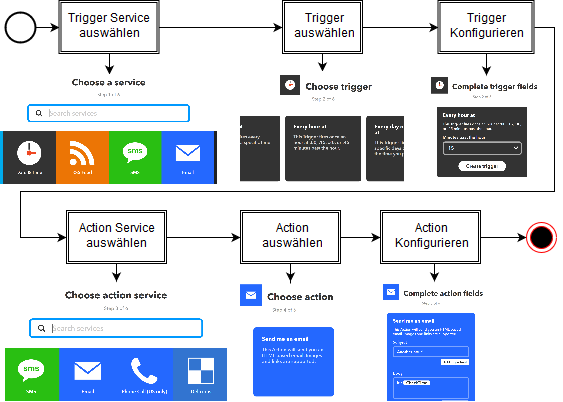
\includegraphics[width=0.9\textwidth]{bilder/chapter2/iftttproz.png}
    \caption{Der Erstellungprozess eines IFTTT-\textit{Recipes}}
    \label{fig:iftttprocess}
\end{figure}
 In Abbildung \ref{fig:iftttprocess} wird der Ablauf zur Erstellung eines IFTTT-Regelsatzes (gennant ''\textit{Recipe}'') dargestellt. Die Erstellung eines \textit{Recipe}, begrenzt sich auf sechs Schritte:
\begin{enumerate}
    \item \textbf{Trigger Service wählen}: Hier wird der Webservice oder das IoT-Gerät gewählt, welches die Quelle für das auszuwertende Trigger-Signal erzeugt. Beispiel: Tageszeit, Sonneneinstrahlung, Wetterdienst;
    \item \textbf{Trigger auswählen}: In diesem Schritt wird die Art des Trigger-Signals definiert. Beispiel für Tageszeit: Wenn X Minuten verstrichen, Jeden Xten Wochentag, von X Uhr bis Y Uhr;
    \item \textbf{Trigger konfigurieren}: Hierbei wird das vorher gewählte Trigger-Signal an die gewünschte Bedingung angepasst. Beispiel: Alle 45 Minuten, Jeden 3ten Wochentag, von 12 Uhr bis 14 Uhr;
    \item \textbf{Action Service wählen}: Analog zum ersten Schritt, wird hier der Konsument des Trigger-Signals in Form eines Webservices oder das IoT-Geräts gewählt. Beispiel: smarte Glühbirne, E-Mail Versand, Thermostat;
    \item \textbf{Action auswählen}: Auch hier wird gleich dem Trigger-Schritt, eine Aktion abhängig vom gewählten Konsument bestimmt. Beispiel: E-Mail versenden, E-Mail Postfach leeren;
    \item \textbf{Action konfigurieren}: Im letzten Schritt, wird die Aktion ausdefiniert. Hierbei werden Daten, die aus dem Trigger-Signal stammen verarbeitet. Beispiel: Sende die Nachricht mit dem Betreff: ''\textit{Es ist <Uhrzeit> Uhr}'';
\end{enumerate}
Aus dem in Abbildung \ref{fig:iftttprocess} gezeigten Recipe entsteht die Regel: Wenn 45 Minuten verstrichen sind, sende eine E-Mail mit dem Betreff: ''Es ist <Uhrzeit> Uhr''. Zwar besitzt eine solche Regel nur geringen Mehrwert, zeigt sie aber auch die Vielseitigkeit dieser Methoden, wenn bedacht wird, dass via IFTTT mehrere Hundert verschiedene Action und Trigger Services miteinander verbinden lässt. Triggers und Actions sind auf jeweils eine pro Recipe limitiert; es ist nicht möglich mehrere Trigger etwa mit bool'schen Operatoren zu verbinden. Auch State-Signale sind prinzipiell nicht statisch. Möchte man bspw. eine Lampe leuchten lassen, solange die Sonne mit Wolken verdeckt ist, muss man dieses \textit{Recipe} in zwei Regeln teilen: ''\textit{Anschalten wenn Wolken}'' und ''\textit{Ausschalten wenn Sonne}'' anstatt ''\textit{Solange Wolken, Lampe anschalten}''.

\paragraph{Bewertung} Der mit Abstand größte Vorteil von IFTTT im Vergleich zu anderen \ac{EUD}-Werkzeugen, ist die geringe Komplexität und vergleichsweise hohe Mächtigkeit. Dies wird dadurch erreicht, dass für eine Vielzahl von \textit{Services}, von professionellen Entwicklern Trigger-Signale und Action-Verhalten definiert wurden. Die Programmierung geschieht in natürlicher Sprache: ''\textit{Wenn dies, dann das}'' und ist daher auch für Laien sehr leicht verständlich. Diese vorteilhafte \textit{Usability} wird auch von mehreren Studien attestiert (\cite{huang2015supporting},\cite{ur2014practical}). 
Natürlich handelt es sich auch bei \ac{TAP} um keine ''\textit{Silver Bullet}'', die sämtliche Probleme von \acp{EUD} im Bereich \ac{IoT} löst. Das signifikanteste Problem ist die geringe Ausdrucksstärke von Regeln, die mit dem vereinfachten Programmierparadigma von bspw. IFTTT einhergeht (\cite{ur2016trigger}). Produkte die \ac{TAP} anwenden sind darauf bedacht, einen Mehrwert zu erzeugen, indem heterogene Systemenlandschaften verbinden können -- nicht aber programmatische Logik der einzelnen Komponente beschreiben. Des Weiteren, hat die Simplifizierung der Programmierung in IFTTT zur Folge, dass das Gefühl von persönlicher Weiterentwicklung mindert. Dies hat die Demotivation des End-Nutzers zur Folge hat (\cite{ur2016trigger}). Ein weiteres Problem ist laut \cite{huang2015supporting} die Mehrdeutigkeit \ac{TAP}-Regeln. Wie sich in der Studie herausstellte, werden selbst einfache Regeln von Nutzern unterschiedlich gedeutet, vor allem wenn eine Aktion eine temporäre Komponente besitzt. Beispielsweise wird ''\textit{Wenn es regnet dann...}'' von manchen Nutzern als ''\textit{Wenn es Beginnt zu regnen dann...}'' und von anderen als ''\textit{Solange es Regnet tue...}'' interpretiert. Das Erörtern solcher Unklarheiten wird zusätzlich erschwert, indem das Auffinden von Fehlern in Regeln von Werkzeugen wie IFTTT schlecht bis gar nicht unterstützt wird.

\subsection{Visuelle Programmierung}\label{subsubsec:samlabs}

\paragraph{Beschreibung} visuelle Programmierung ist per se keine \ac{EUD}-Technik sondern vielmehr eine abstrakte Darstellungsform für Programmcode. Visuelle Programmiersprachen (VPS) \acused{VPS} erlauben es dem Benutzer, durch die Erstellung und Manipulation von visuellen Objekten Programmcode zu generieren. Durch das Benutzen von visuellen statt textuellen Objekten, erhofft man sich, die Daten, Abläufe und Softwarefragmente für den End-Nutzer begreifbarer zu machen und somit die Benutzerfreundlichkeit als Ganzes zu verbessern (\cite{burnett2002software}). \ac{VPS} ermöglichen diese Begreifbarkeit durch die gezielte Verwendung von Metaphern: Blöcke, Röhren, Graphen, usw. sind alltägliche Elemente, welche sich durch ihre Verhalten, Struktur und Benutzung charakterisieren. Durch den gezielte Einsatz solcher Analogien, erhofft man sich das mentale Modell des Endnutzers zu prägen (\cite{Myers1986vis}). In der Praxis sind \acp{VPS} weit verbreitet: von der Erzeugung komplexer Funktionen (bspw. LabVIEW) über die Programmierung von Computerspiel Logik (bspw. Unreal-Engine Blueprint\footnote{\url{https://docs.unrealengine.com/en-us/Engine/Blueprints} -- besucht September 2018}), bis hin zur Steuerung von sowjetischen Raumfähren (bspw. DRAKON \cite{parondzhanov1995drakon}) unterstützen \acp{VPS} Domänenexperten, bei der Erstellung von Softwareartefakten. 

\paragraph{Funktionsweise} Eine einzige Funktionsweise für \ac{VPS} gibt es aufgrund der breit gefächerten Anwendungsgebiete nicht. Grundsätzlich erhofft man sich durch das Einführen zusätzlicher Informationsdimension (bspw. Position, Farbe, Animation), die Benutzerfreundlichkeit für den Endnutzer zu verbessern (\cite{Myers1986vis}). Es lassen sich allerdings verschiedene Aspekte identifizieren, welche prägend für das Design einer \ac{VPS} sind: Visualisierung von Kontrollfluss und/oder Datenfluss, des Programmzustands, Funktionsumfang und Programmstruktur (\cite{boshernitsan2004visual}). Grundsätzlich unterscheiden sich \acp{VPS} nicht von \acp{DSL}. Sie bestehen auch aus einer Syntax von Elementen und einer Semantik die den Elementen Sinn verleiht. Zusätzlich besitzen \ac{VPS} oftmals Pragmatismen -- unter ihnen versteht man spezielle Funktionalitäten zur Verbesserung der Usability; beispielsweise das manuelle modifizieren von Variablen zur Laufzeit des Programms (\cite{Repenning2017MovingBS}). Kernstück einer einer \ac{VPS} ist die Metapher, mit welcher der Programmcode abstahiert wird. 

\paragraph{SAM Labs/Studio} SAM Labs ist ein Bildungswerkzeug für \ac{IoT}. Es besteht -- ähnlich wie cBlocks -- aus einer Sammlung von separaten Sensor- und Aktorblöcken, welche kabellos miteinander kommunizieren. Jeder Block (Abbildung \ref{fig:samlabssub1}) besitzt nur eine Aufgabe: Fühlen von Temperatur, Auslesen von elektrischem Widerstand, Leuchten von LEDs, Abspielen eines Geräusches, etc. 

\begin{figure}[h]
\centering
\begin{subfigure}{.5\textwidth}
  \centering
  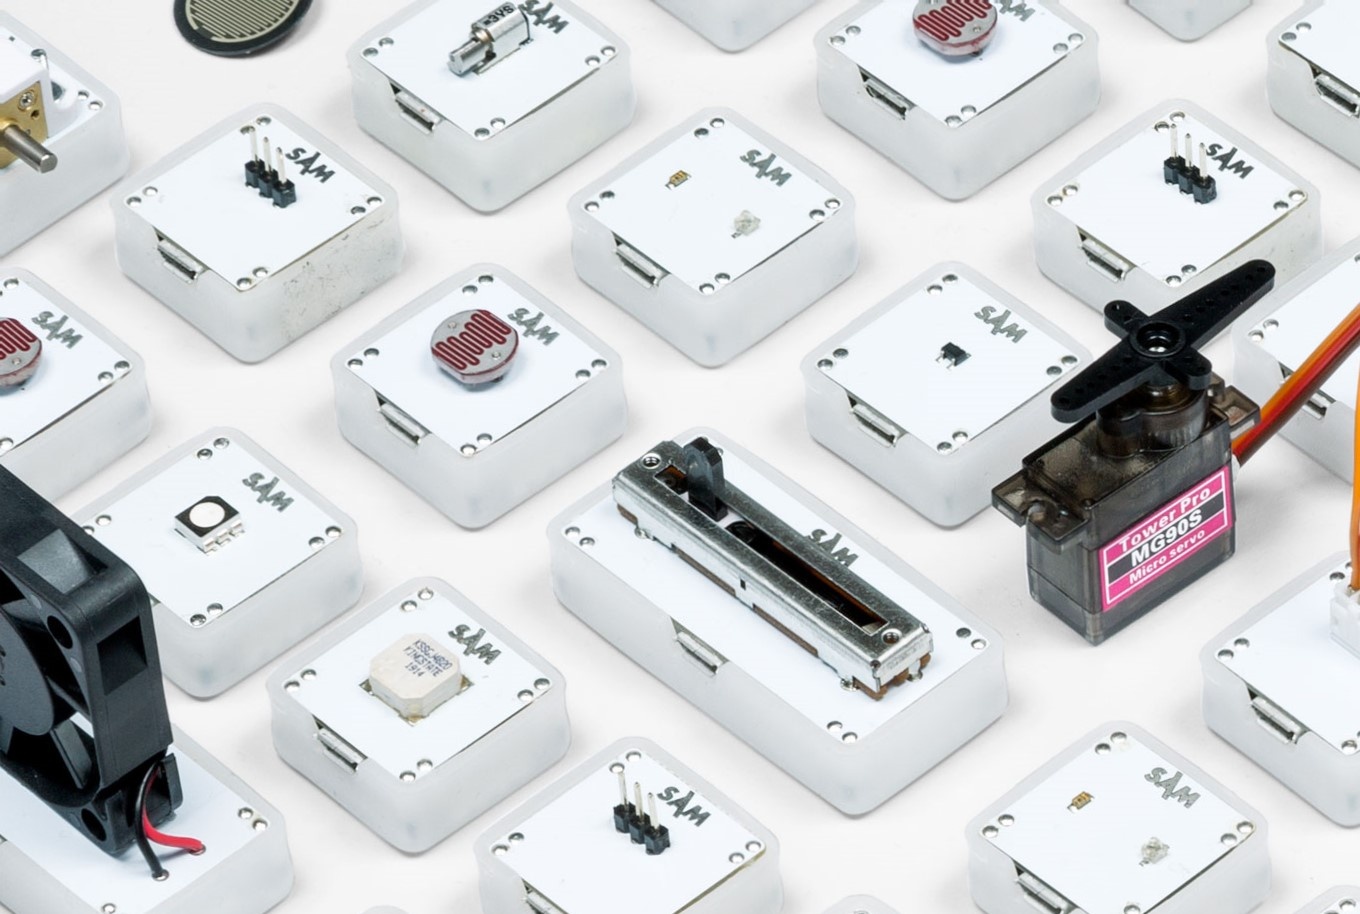
\includegraphics[width=.9\linewidth]{bilder/chapter2/samlabs.jpg}
  \caption{Eine Sammlung von SAM Labs Blöcken}
  \label{fig:samlabssub1}
\end{subfigure}%
\begin{subfigure}{.5\textwidth}
  \centering
  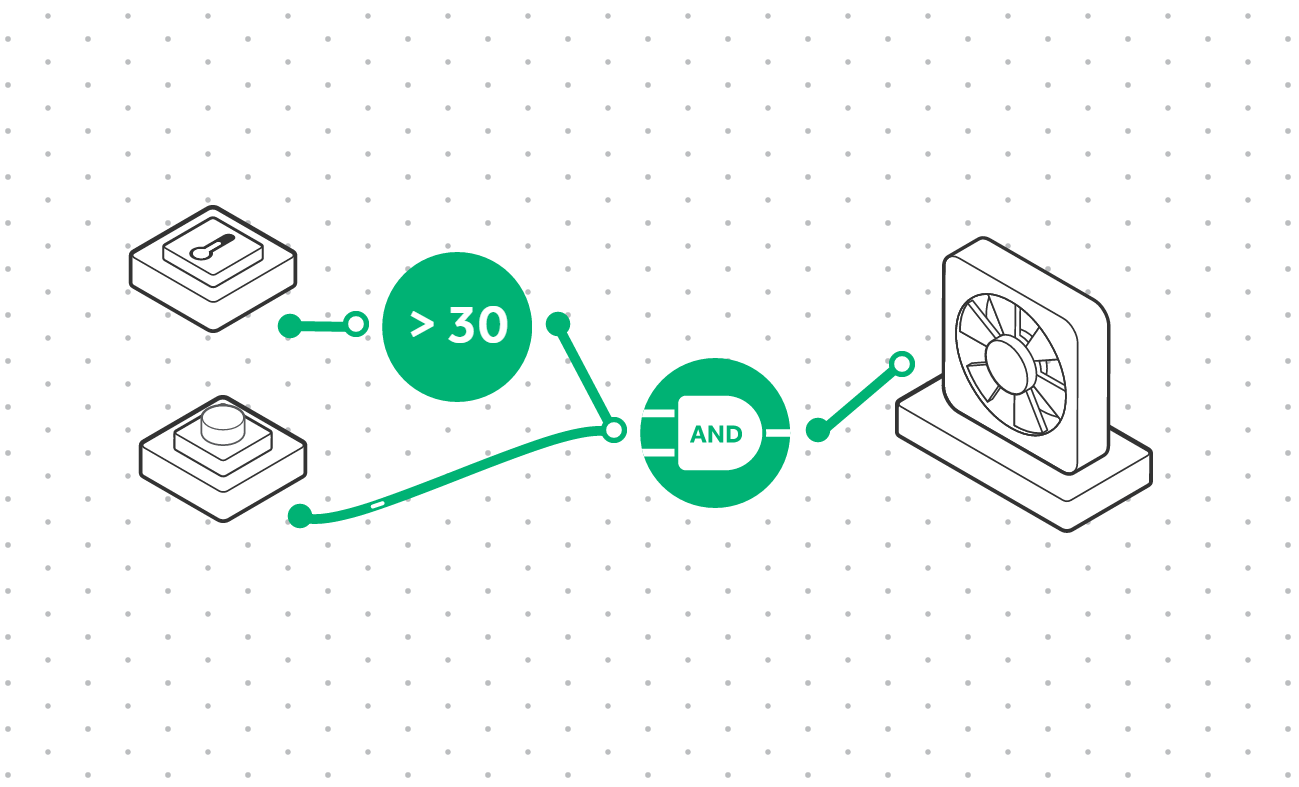
\includegraphics[width=.9\linewidth]{bilder/chapter2/samlabside.png}
  \caption{Beispielprogramm entworfen in Sam Studio}
  \label{fig:samlabssub2}
\end{subfigure}
\caption{Das SAM Labs Ökosystem besteht aus Funktionsblöcken (links) und der SAM Studio IDE zur Erstellung der Programmlogik (rechts)}
\label{fig:samlabs}
\end{figure}

Das \ac{EUD}-Werkzeug, welches Sam Labs Nutzern erlaubt Programme zu erstellen heißt \textbf{Sam Studio}. Kernstück bei der Programmierung stellen hierbei drei Arten von Nodes: Signalquellen (Sensoren, Interaktionen, etc.), Wandler (Bool'scher Operator, Arithmetischer Operator, etc.) und Signalkonsumenten (Webservices, Aktoren). Jede Node besitzt jeweils einen Input und/oder einen Ouput über welches die Node ein Signal sendet oder empfangen kann. Inputs und Outputs werden mit einer Drag-n-Drop Geste miteinander über Links verbunden werden. Diese Links stellen dauerhafte Kommunikationskanäle zwischen den Nodes dar, analog zu Funktionsaufrufen zwischen verschiedenen Objekten. Sensoren zeichnen sich durch ihre skeuomorphische Darstellung aus, der Existenz eines Outputs und dem Fehlen eines Inputs. Aktoren besitzen ebenso eine realitätsnahe Darstellung, allerdings umgekehrt zum Sensor kein Ouput, dafür aber einen Input. Wandler besitzen einen Input und Output und eine abstrakte Darstellung, welche zusätzliche Information zur Konfiguration dessen liefert. In Bild \ref{fig:samlabssub2} ist ein Beispielsprogramm, welches aus zwei Sensoren (Temperatur und Button), zwei Wandlern (Komperator und Bool'sches Gatter) und einem Aktor (Ventilator) besteht. Dieses simple Programm drückt folgende Logik aus: ''\textit{Solange Temperatur >30°C und der Schalter gedrückt ist, rotiere den Ventilator}''. Anzumerken an der Darstellung ist, dass es nicht ersichtlich ist, welche Daten zwischen den Nodes fließen ob dies Steuerungs- oder Datensignale sind, ist nicht erkenntlich. 

\paragraph{Beurteilung} Graphische Programmierschnittstellen genießen neben \ac{TAP} die höchste Popularität als \ac{EUD}-Werkzeug im \ac{IoT}-Bereich. SAM Studio ist hierfür ein prominentes Beispiel, an dem man die Vor- und Nachteile des Paradigmas erläutern kann. Der primäre und offensichtlichste Vorteil von visuellen Programmiersprachen liegt in der Darstellung selbst. Menschen haben eine visuelle Denkweise, daher ist es naheliegend Probleme und Lösungen auf einer visuellen Ebene darzustellen, statt einer textuellen. Visuelle Metaphern erlauben es Endnutzern Erfahrungen aus der realen Welt auf die Programmierung übertragen. In SAM Studio werden Links zwischen den datenverarbeiteten Elementen gezogen. Dies könnte man mit dem ziehen von Förderbändern zwischen materialverarbeitenden Maschinen in der reellen Welt vergleichen. Des Weiteren lädt SAM Studio durch das einfache Manipulieren und Kopieren von einzelnen Elementen ein, explorative Entwicklung zu betreiben. Darüber hinaus, erleichtert die Darstellung von SAM Studio das \textit{Debugging} von Prototypen. Hierfür werden Animationen verwendet, durch die sich der Datenfluss visuell nachverfolgen lässt. Ein Vorteil im Vergleich zu \ac{TAP}, ist die Darstellung paralleler Datenströme. Wie in Bild \ref{fig:samlabssub2} zu sehen ist, sind die asynchron Signale der Datenquellen graphisch nachvollziehbar. Diese verteilte Erzeugung und Verarbeitung von Events ist schwierig in textueller Form darzustellen. 

\ac{VPS} besitzt nicht nur Vorteile. Eine der prominentesten Kritiken gegenüber \acp{VPS} wurde von Peter L. Deutsch (\cite{MASON201368}) formuliert:

\begin{quote}
    ''\textit{The problem with visual programming is that you can’t have more than 50 visual primitives on the screen at the same time.}''
\end{quote}


Diese Kritik bezieht sich auf die relativ niedrige Informationsdichte von \acp{VPS} im Vergleich zu textuellen Programmiersprachen, wenn man davon ausgeht, dass maximal 50 visuelle Elemente auf einmal auf einen Computerbildschirm passen. Allerdings wurde diese Aussage zumindest Teilweise entschärft unter dem Gesichtspunkt, dass ähnliche Konzepte wie Komposition und Dekomposition von elementaren Komponenten, um komplexere Elemente zu schaffen auf \ac{VPS} übertragbar ist.

SAM Studio hat speziell noch folgende Nachteile:
\begin{itemize}
    \item \textbf{Geringer Funktionsumfang}: Der Funktionsumfang ist zweierlei begrenzt: zum einen, gibt es nur eine geringe Anzahl von SAM Labs Blöcke. Der Endnutzer hat dadurch nur eine begrenzte Anzahl von möglichen Sensordaten und Aktor-Aktionen zur Verfügung. Zusätzlich ist die Ansteuerung von Nodes hart vordefiniert. Der Lüfter aus Bild \ref{fig:samlabssub2} lässt sich nur binär ansteuern; möchte man bspw. die Lüfterdrehzahl analog regeln ist dies nicht möglich. Dies wird zusätzlich dadurch erschwert, dass keine Komponente von SAM Labs \textit{Open Source} ist und somit nicht modifizierbar werden kann.
    \item \textbf{Vermischung von Datenfluss und Kontrollfluss} Die Link Metapher von SAM Studio ist nicht in allen Fällen konsistent. In manchen Fällen, wie in Bild \ref{fig:samlabssub2}, wird ein Kontrollfluss zur Steuerung des Lüfters modelliert. Allerdings können Links aber auch Datenflüsse darstellen, bspw. ist das übermitteln von Farbcodes zwischen einem Wandler und einem Aktor möglich. Solche Inkonsistenzen hemmen das Verständnis von Programmen in SAM Studio.
    \item \textbf{Fehlende Fehlerprävention} Grundsätzlich kann der Nutzer sämtliche Nodes miteinander verbinden. SAM Studio erlaubt es somit auch, unsinnige Kombinationen zu erzeugen (z.B. Farbcodes an Ventilator senden). Dies kommt gleich einer Programmiersprache ohne statische Typisierung. Fehlerprävention wird somit nicht betrieben und zwingt den Nutzer sein Programm erst zur Laufzeit manuell zu validieren.
\end{itemize}
Da es sich bei SAM Labs um ein Produkt für Schulkinder zwischen sieben und zwölf Jahren handelt, ist die extreme Simplifizierung des Programmiermodells nachvollziehbar. 

\subsection{Zusammenfassung}
Zusammenfassend ist zu sagen, dass es viele Möglichkeiten gibt \ac{EUD} für \ac{IoT} umzusetzen. Die Vielfalt an Ansätzen und die Fokussierung von Forschung (\cite{2015iseud}, \cite{2017iseud}, uvm.) auf dieses Thema ist Zeuge dessen Relevanz. Unabhängig der Ansätze, sind sich die Autoren einig, dass die immerzu wachsende Digitalisierung unseres Alltagslebens durch \textit{Smart Objects} einem Mangel an Softwareingenieuren gegenübersteht, welche die Nischenbedürfnisse von Endnutzern umsetzen können. \acp{EUD} erlauben es diesen Mangel durch benutzerfreundliche Programmierschnittstellen zu überbrücken.

Wie sich in den vorherigen Unterkapiteln ableiten lässt, kommt es bei dem Design von \acp{EUD}-Werkzeugen auf drei Kriterien an: Scope, Endnutzer und Anwendungsdomäne. Der \textbf{Scope}, welcher die Balance zwischen Abbildungsvermögen der \ac{EUD} und der Komplexität der Darstellung der Programmartefakte definiert, kann extrem Unterschiedlich sein. IFTTT und SAM Labs setzen ihr Hauptaugenmerk auf Simplizität in allen Bereichen legen. Dies lässt sich durch die Anwendungsdomäne der \ac{EUD}-Systeme erklären: SAM Labs ein Werkzeug ist, um die Grundlagen von \textit{MINT}-Bildung Schülern näher zu bringen (hoher Usability-Anspruch, geringer Funktionsumfang). An dieser Stelle ist allerdings anzumerken, dass auch \ac{EUD}-Werkzeuge existieren (bspw. LabVIEW\footnote{\url{http://www.ni.com/de-de/shop/labview.html} -- besucht September 2018}), die von Ingenieuren im Alltag verwendet um komplexe Transformationen von Daten visuell darzustellen (geringerer Usability-Anspruch, hoher Funktionsumfang). Der \textbf{Endnutzer} selbst ist natürlich ein weiteres zentrales Kriterium für das Design des \ac{EUD}. Der Endnutzer nimmt mit seinen Zielen, seinem technischen Verständnis und seinem mentalen Modell, Einfluss auf die Anforderungen des \ac{EUD}-Werkzeugs, hinsichtlich Darstellung und Komplexität. IFTTT beispielsweise versucht es mit seinem natürlichsprachlichen Ansatz und definieren möglichst viele Aktionen vor, um auch Nutzern programmieren zu ermöglichen, die keinerlei Interesse an der Programmierung selbst besitzen. Die \textbf{Anwendungsdomäne} selbst ist von großer Bedeutung für die Wahl des \ac{EUD}-Paradigmas. \ac{IoT}-Lösungen charakterisieren sich als Event-getriebene, parallele System, welche (physisch) geteilte Teilsysteme miteinander verbinden (siehe Kapitel \ref{subsubsec:wsan}). Während die Event-Komponente bei IFTTT durch Regeln dargestellt wird, verwendet SAM Labs eine Röhren-Metapher um den parallelen Daten- und Kontrollfluss zu visualisieren. Beide Darstellungsarten haben Vor- und Nachteile hinsichtlich abbildbarer Komplexität und Usability. Nicht jedes \ac{EUD}-Paradigma ist allerdings für die Anwendungsdomäne \ac{IoT} sinnvoll anwendbar. \ac{PBD} bspw. fokussiert sich darauf dem Computer sequentielle, repetitive Schritte, die der Endnutzer manuell ausführt, nachzuahmen. Die Anwendungsdomäne ist somit ein weiterer Grund, die Metapher der Darstellung sorgfältig zu wählen.

Eine \ac{EUD}-Umgebung sollte die oben genannten Punkte berücksichtigen. Im Falle dieser Thesis der Scope des Prototyping definiert, die \textit{Persona} des Endnutzers charakterisiert und die Anwendungsdomäne geklärt werden.
